\documentclass[a4paper,12pt,twoside,openright]{report}

\usepackage[pdfborder={0 0 0}]{hyperref}    % turns references into hyperlinks
\usepackage[margin=25mm]{geometry}  % adjusts page layout
\usepackage{graphicx}  % allows inclusion of PDF, PNG and JPG images
\usepackage{verbatim}
\usepackage{pdfpages}  % to embed proposal at the end of the dissertation
\usepackage{textcomp}

\renewcommand{\baselinestretch}{1.1}    % adjust line spacing to make
% more readable

\begin{document}
	
	\bibliographystyle{plain}
	
	
	%%%%%%%%%%%%%%%%%%%%%%%%%%%%%%%%%%%%%%%%%%%%%%%%%%%%%%%%%%%%%%%%%%%%%%%%
	% Title
	
	
	\pagestyle{empty}
	
	\rightline{\LARGE \textbf{Peter Lotts}}
	
	\vspace*{60mm}
	\begin{center}
		\Huge
		\textbf{Adding network subsystem provenance collection to CADETS} \\[5mm]
		Computer Science Tripos -- Part II \\[5mm]
		Downing College \\[5mm]
		\today  % today's date
	\end{center}
	
	%%%%%%%%%%%%%%%%%%%%%%%%%%%%%%%%%%%%%%%%%%%%%%%%%%%%%%%%%%%%%%%%%%%%%%%%%%%%%%
	% Proforma, table of contents and list of figures
	
	\pagestyle{plain}
	
	\chapter*{Proforma}
	
	{\large
		\begin{tabular}{ll}
			Name:               & \bf Peter Lotts                       \\
			College:            & \bf Downing College                     \\
			Project Title:      & \bf Adding network subsystem provenance \\
								& \bf collection to CADETS \\
			Examination:        & \bf Computer Science Tripos -- Part II, 2018  \\
			Word Count:         & \bf tbc\footnotemark[1]  \\
			Project Originator: & Dr R.~Sohan                    \\
			Supervisor:         & Dr G.~Jenkinson                    \\ 
		\end{tabular}
	}
	\footnotetext[1]{This word count was computed at [date]	by the provided online tool at \texttt{URL}
	}
	\stepcounter{footnote}
	
	
	\section*{Original Aims of the Project}
	
	To provide additional metadata collection tools for network packets to the Computer Laboratory's existing CADETS project. This will be provided by tracking individual packets as they flow through the network stack of the FreeBSD\footnote{\texttt{http://www.freebsd.org/}} kernel, and making information regarding memory locations used and the time taken by each layer to process a given packet available to DTrace\footnote{\texttt{http://dtrace.org/}}. DTrace is a generic Dynamic Tracing framework which is the primary data collection tool used by the CADETS project to bring kernel data into userspace for analysis. The performance impact of the project on network packet delivery is to be evaluated.
	
	
	\section*{Work Completed}
	
	\textit{What we actually did.}
	
	\section*{Special Difficulties}
	
	None. [We hope!!]
	
	\newpage
	\section*{Declaration Of Originality}
	
	I, Peter Lotts of Downing College, being a candidate for Part II of
	the Computer Science Tripos, hereby declare
	that this dissertation and the work described in it are my own work,
	unaided except as may be specified below, and that the dissertation
	does not contain material that has already been used to any substantial
	extent for a comparable purpose.
	
	\bigskip
	\leftline{Signed [signature]}
	
	\medskip
	\leftline{Date [date]}
	
	\tableofcontents
	
	\listoffigures
	
	%%%%%%%%%%%%%%%%%%%%%%%%%%%%%%%%%%%%%%%%%%%%%%%%%%%%%%%%%%%%%%%%%%%%%%%
	% now for the chapters
	
	\pagestyle{headings}
	
	\chapter{Introduction}
	
	\section{Background [Use Case?]}
	
	Nowadays, most cyberattacks from nation state actors do not take on the traditional form of a piece	of malware which tries to find a store of sensitive data and dump it back to the attacker as quickly as	possible before system administrators have time to intervene. Instead, these attacks slowly 	infiltrate the target system, hiding out of sight and learning the use patterns of normal users. They then exploit this knowledge to slowly make horizontal transfers within the target enterprise’s internal	network, and extract sensitive data from databases in such a way that the access is hard to	distinguish from normal access. Such an attack is called an Advanced Persistent Threat (APT), and can go on for months or years without system administrators realising. Eventually, it is likely that the malware will make a mistake and trigger an indicator of compromise to be observed by administrators, but by then it is difficult to tell when and how the malware entered the system, and what data it has seen. This can make impact assessments, as well as efforts to prevent a similar attack in future, very difficult.
	
	The Computer Laboratory has a project which is trying to combat this by building CADETS, a Causal, Adaptive, Distributed, and Efficient Tracing System, on top of the FreeBSD operating system. The system is being built to track the provenance of data by collecting metadata from computers all over the network about what processes act on what data and when. This metadata is then collected in a distributed database, where it can be analysed to trace data flows throughout the computer system. This should allow analysts to trace malware back to possible entry times and methods, which they can then analyse further.
	
	This project will add support for collecting metadata on network packets as they flow through the kernel	network stack. The data collected will allow users of CADETS to seek out suspicious activity which may be being used to attack a system, and will be able to provide a list of locations in kernel memory where packet data were stored. The latter allows a rapid impact assessment to be produced if a system administrator is able to determine that some malicious code had access to a particular set of kernel memory addresses, as CADETS will let the administrator infer what data may have been leaked.
	
	\section{The Network Stack}
	
	Provide a brief explanation of the concept of the network stack up to the socket API, layering, fragmentation etc.
	
	\section{Tracing as a Security Tool}
	
	Discuss why CADETS is useful, point out that we can't generally assume the security of a system to be perfectly watertight (Meltdown/Spectre), and the need for something to pick up the pieces later.
	
	\section{Similar Work}
	
	Just need to mention Resourceful? - I haven't used it so far, is it even relevant?
	
	\section{Overall design}
	
	The project is to assign uniquely identifying tags to each packet as it flows through the network stack, noting that packet fragmentation/reassembly will make this more difficult. This will then allow DTrace tracepoints to read the tag on each packet when an interesting operation (broadly speaking, a memory allocation) is performed on it. From here, scripts written in DTrace's D language will be able to forward information to the CADETS userspace application for processing.

	
	
	\chapter{Preparation}
	
	\section{Starting Point}
	
	The CADETS project currently has a user-space application which collects metadata on kernel-level	datastructures via libdtrace, translates the metadata to a JSON format for easy interpretation, and	then sends this away for processing (often over the network). It also has an application with a user interface to display the data it has collected.
	
	The FreeBSD kernel provides a means of tagging its main internal structure of interest, namely \verb|struct mbuf| using \verb|struct mbuf_tags|. It is thought that this will be sufficient to tag a packet’s data with an unique identifier in order to track its progress through the kernel’s network stack.
	
	Under Linux, the Resourceful framework is able to collect data from auto-generated tracepoints	within the Linux kernel with relatively low overhead, but it does not currently inspect the network subsystem.
	
	\section{Installing the Development System}
	
	I had no prior experience with FreeBSD usage or development, so the first challenge was to get a system up and running to be used for both development and testing. I decided to host FreeBSD as a virtual machine on my Windows 10 laptop, as it has reasonable performance for compiling code, whilst being portable and allowing me to work on the project wherever I am. The virtual machine was set up using Oracle\texttrademark\ VM VirtualBox\footnote{\texttt{http://www.virtualbox.org/}}, as I have most experience using this virtualisation application.
	
	The FreeBSD website provides preinstalled images\footnote{\texttt{http://www.freebsd.org/where.html\#download}} for various virtual machine types, and I decided to use one of these as a basis due to my inexperience with the operating system. Only slow progress was made during the first few days of using this new operating system, as the preinstalled images have a rather basic toolset available and I had to learn how to use a new package manager, and the FreeBSD `ports' system. Having acclimatised to these, I was able to fork the CADETS custom kernel, build and install it onto the running machine.
	
	\section{FreeBSD kernel study}
	
	The first significant piece of planned project work was to inspect the FreeBSD kernel source code for the network stack, gain some familiarity with it, and note the locations of operations which are of particular interest to the project, either from a packet tagging perspective or from the perspective of packet data being copied to a new memory location.
	
	The study commenced at the point where outgoing packets enter the IP layer of the network stack, namely the top of the \verb|ip_output| function. From here, the packet was followed down through the IP layer, exploring all possible control paths
	\footnote{
		With one or two notable exceptions, namely that
		\begin{itemize}
			\item Berkley Packet Filter (BPF) was considered to be out of scope for the project
			\item IPSec allows arbitrary code to be executed via its `hooks' system, and so this cannot be inspected
		\end{itemize}
	}
	and possible exit routes into lower layers. Once the packets had left to go to device drivers, the study then turned to the \texttt{netisr} system, which is responsible for receiving packets from device drivers in the FreeBSD kernel and handing them on to the appropriate next layer (usually the IP layer) to be processed. From here, packets were followed back up the network stack in a similar manner, up to the end of \verb|ip_input|, where packets leave the IP layer to go to the next layer up.
	
	At this point, it was noticed that the project was getting a little behind schedule and, in a meeting with my supervisor, it was decided that for the moment the project would not look any higher than the IP layer, as there was no significant academic benefit to be gained from continuing up to look at the TCP layer. This could be completed at a later stage in the project if time became available.
	
	DID WE GET TIME FOR THIS?
	
	
	\chapter{Implementation}
	
	
	\chapter{Evaluation}
	
	
	\chapter{Conclusion}
	
	
	
	%%%%%%%%%%%%%%%%%%%%%%%%%%%%%%%%%%%%%%%%%%%%%%%%%%%%%%%%%%%%%%%%%%%%%
	% the bibliography
	\addcontentsline{toc}{chapter}{Bibliography}
	\bibliography{refs}
	
	%%%%%%%%%%%%%%%%%%%%%%%%%%%%%%%%%%%%%%%%%%%%%%%%%%%%%%%%%%%%%%%%%%%%%
	% the appendices
	\appendix
	
	
	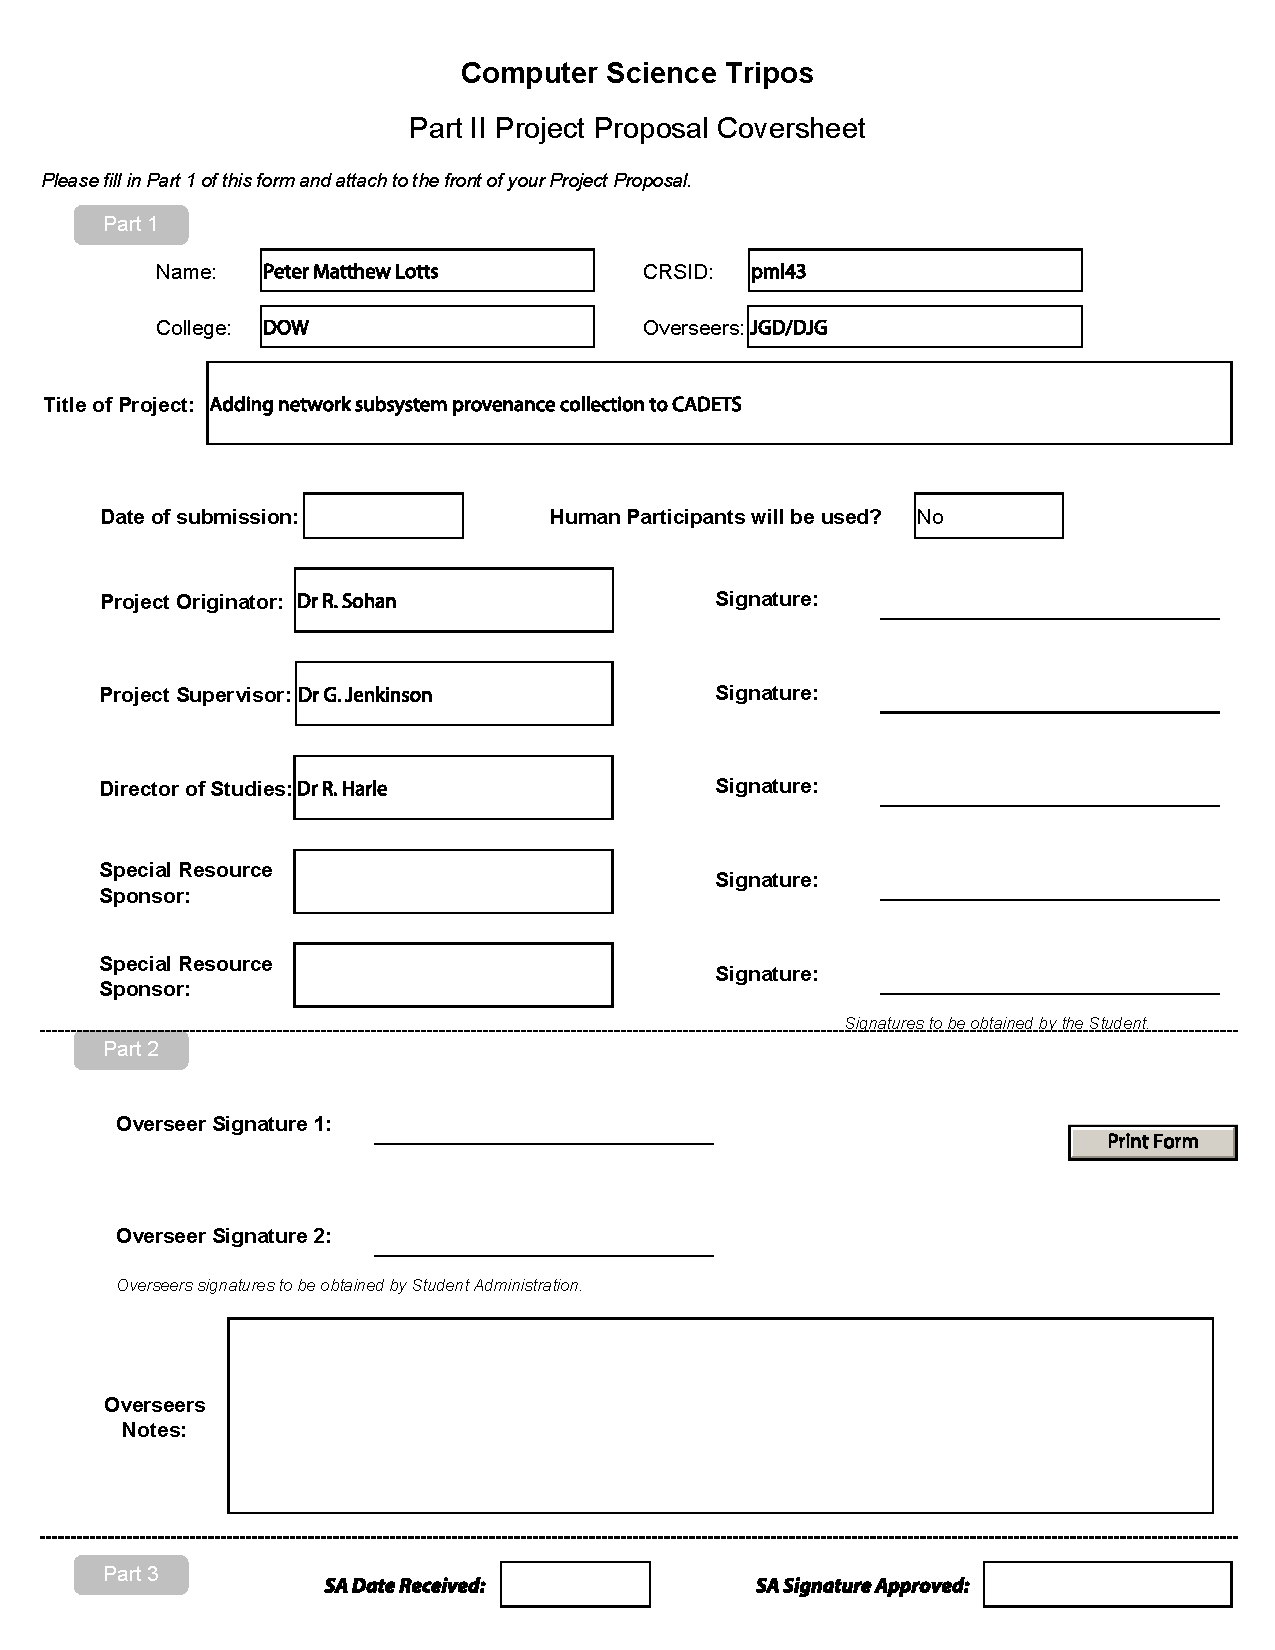
\includepdf{include/Project-Proposal-Cover-Sheet.pdf}
	\includepdf[pages={2-}]{include/Project-Proposal.pdf}
	
	
\end{document}
